%%%%%%%% ICML 2018 EXAMPLE LATEX SUBMISSION FILE %%%%%%%%%%%%%%%%%

\documentclass{article}

% Recommended, but optional, packages for figures and better typesetting:
\usepackage{microtype}
\usepackage{graphicx}
\usepackage{subfigure}
\usepackage{amsmath}
\usepackage{booktabs} % for professional tables


% hyperref makes hyperlinks in the resulting PDF.
% If your build breaks (sometimes temporarily if a hyperlink spans a page)
% please comment out the following usepackage line and replace
% \usepackage{icml2018} with \usepackage[nohyperref]{icml2018} above.
\usepackage{hyperref}

% Attempt to make hyperref and algorithmic work together better:
\newcommand{\theHalgorithm}{\arabic{algorithm}}

% Use the following line for the initial blind version submitted for review:
\usepackage{icml2018}

% If accepted, instead use the following line for the camera-ready submission:
%\usepackage[accepted]{icml2018}

% The \icmltitle you define below is probably too long as a header.
% Therefore, a short form for the running title is supplied here:
\icmltitlerunning{Compressive Sensing with Low Precision Data Representation: Radio Astronomy and Beyond}

\begin{document}
\onehalfspacing
\onecolumn
\icmltitle{Supplementary Material for Compressive Sensing with Low Precision Data Representation: Radio Astronomy and Beyond}

% It is OKAY to include author information, even for blind
% submissions: the style file will automatically remove it for you
% unless you've provided the [accepted] option to the icml2018
% package.

% List of affiliations: The first argument should be a (short)
% identifier you will use later to specify author affiliations
% Academic affiliations should list Department, University, City, Region, Country
% Industry affiliations should list Company, City, Region, Country

% You can specify symbols, otherwise they are numbered in order.
% Ideally, you should not use this facility. Affiliations will be numbered
% in order of appearance and this is the preferred way.

% find helpful for describing your paper; these are used to populate
% the "keywords" metadata in the PDF but will not be shown in the document


\vskip 0.3in


% this must go after the closing bracket ] following \twocolumn[ ...

% This command actually creates the footnote in the first column
% listing the affiliations and the copyright notice.
% The command takes one argument, which is text to display at the start of the footnote.
% The \icmlEqualContribution command is standard text for equal contribution.
% Remove it (just {}) if you do not need this facility.

%\printAffiliationsAndNotice{}  % leave blank if no need to mention equal contribution
%\printAffiliationsAndNotice{\icmlEqualContribution} % otherwise use the standard text.

\section{Proofs}
We begin with introducing our notation.
\begin{enumerate}
    \item ${\bf y} = {\bf \Phi} {\bf x} + {\bf e} = {\bf \Phi} {\bf x}^s + {\bf \Phi}({\bf x}-{\bf x}^s) + {\bf e}$,
    \item $\boldsymbol{\varepsilon} = {\bf \Phi}({\bf x}-{\bf x}^s) + {\bf e}$, hence ${\bf y} = {\bf \Phi} {\bf x}^s + \boldsymbol{\varepsilon}$,
    \item $\boldsymbol{\epsilon_y} = Q({\bf y},b) - {\bf y}$,
    \item $\Gamma^{[n]} = \rm{supp}\{{\bf x}^{[n]} \}$, $\hat{\Gamma}^{[n]} = \rm{supp}\{\hat{{\bf x}}^{[n]} \}$ and $\Gamma^{*} = \rm{supp}\{{\bf x}^{*} \}$,
    \item $B^{[n]} = \Gamma^{[n]} \cup \Gamma^{*}$ and $B^{[n]} = \hat{\Gamma}^{[n]} \cup \Gamma^{*}$,
    \item ${\bf a}^{[n+1]} = \hat{{\bf x}}^{[n]} + \mu^{[n]}{\bf \Phi}^{\dag}({\bf y} - {\bf \Phi}\hat{{\bf x}}^{[n]})$ and $\hat{{\bf a}}^{[n+1]} = \hat{{\bf x}}^{[n]} + \hat{\mu}^{[n]}Q_{1}({\bf \Phi})^{\dag}({\bf y} - Q_2({\bf \Phi})\hat{{\bf x}}^{[n]})$,
    \item ${\bf x}^{[n+1]} = H_s({\bf a}^{[n+1]})$ and $\hat{{\bf x}}^{[n+1]} = H_s(\hat{{\bf a}}^{[n+1]})$,
    \item ${\bf r}^{[n]} = \hat{{\bf x}}^{[n]}-{\bf x}^s$.
\end{enumerate}
Assume $\mathbf{\bf \Phi}$ satisfies the non-symmetric Restricted Isometry Property 
\begin{equation}\label{rip}
\alpha_{s} \leq \frac{\|{\bf {\bf \Phi}} {\bf x}\|_2}{\|{\bf x}\|_2} \leq \beta_{s}
\end{equation}
for all ${\bf x}: \|{\bf x}\|_0 \leq s$, and some $\alpha_s, \beta_s \in \mathbb{R}$ such that $0<\alpha_s\leq \beta_s$. the so-called restricted isometric constants. Inherent from its definition, the restricted isometry holds for the quantized measurement matrix denoted by $Q({\bf {\bf \Phi}}, b_m)$ such that
\begin{equation}\label{rip_lowprecision}
\hat{\alpha}_{s} \leq \frac{\|Q({\bf {\bf \Phi}}, b_m) {\bf x}\|_2}{\|{\bf x}\|_2} \leq \hat{\beta}_{s}
\end{equation}
where $\hat{\alpha}_{s}$ and $\hat{\beta}_{s}$ are associated restricted isometry constants. For simplicity, we drop $b_m$, and use $Q({\bf {\bf \Phi}})$ instead. Also, let $\gamma_s=\beta_s/\alpha_s-1$ and $\hat{\gamma}_s=\hat{\beta}_s/\hat{\alpha}_s-1$.

\begin{remark}
The adaptive setting of step size parameter $\mu^{[n]}$ and $\hat{\mu}^{[n]}$ in normalized IHT is shown to satisfy
\begin{equation}\label{bounds_mu}
   1/\beta^2_{2s} \leq \mu^{[n]} \leq 1/\alpha^2_{2s},
\end{equation}
\begin{equation}\label{bounds_muhat}
   1/\hat{\beta}^2_{2s} \leq \hat{\mu}^{[n]} \leq 1/\hat{\alpha}^2_{2s}.
\end{equation}
\end{remark}


We will start by the following results.
\begin{lemma}\label{lemmas_on_phi}
{\rm{\cite{blumensath2010niht}}}
If ${\bf {\bf \Phi}}$ satisfies the restricted isometry property, then for $|\Gamma|\leq 2s$
\begin{equation}\label{mu*phi}
    \| {\bf {\bf \Phi}}_{\Gamma}^T{\bf x}\|_2 \leq \beta_{2s}\|{\bf x} \|_2,
\end{equation}
\begin{equation}\label{mu*phi*phi}
    \| \mu^{[n]}{\bf {\bf \Phi}}_{\Gamma}^T{\bf {\bf \Phi}}_{\Gamma}{\bf x}_{\Gamma}\|_2 \leq (\gamma_{2s}+1)\|{\bf x}_{\Gamma} \|_2,
\end{equation}
\begin{equation}\label{1-mu*phi*phi}
    \| ( {\bf I}- \mu^{[n]}{\bf {\bf \Phi}}_{\Gamma}^T{\bf {\bf \Phi}}_{\Gamma}){\bf x}_{\Gamma}\|_2 \leq \gamma_{2s}\|{\bf x}_{\Gamma} \|_2,
\end{equation}
\begin{equation}\label{mu*phi1*phi2}
     \| \mu^{[n]}{\bf {\bf \Phi}}_{\Upsilon}^T{\bf {\bf \Phi}}_{\Lambda}{\bf x}_{\Lambda}\|_2 \leq \gamma_{2s}\|{\bf x}_{\Lambda} \|_2,
\end{equation}
where $\Upsilon$ and $\Lambda$ are two disjoint sets (i.e., $\Upsilon \cap \Lambda = \emptyset$) such that $|\Upsilon \cup \Lambda| \leq 2s$. 
\end{lemma}
Clearly, similar results hold for $Q(\boldsymbol{{\bf \Phi}})$ such that
\begin{equation}\label{q_mu*phi}
     \|Q({\bf {\bf \Phi}})_{\Gamma}^T{\bf x}\|_2 \leq \hat{\beta}_{2s}\|{\bf x} \|_2,
\end{equation}
\begin{equation}\label{q_mu*phi*phi}
    \| \mu^{[n]}Q({\bf {\bf \Phi}})_{\Gamma}^TQ({\bf {\bf \Phi}})_{\Gamma}{\bf x}_{\Gamma}\|_2 \leq (\hat{\gamma}_{2s}+1)\|{\bf x}_{\Gamma} \|_2,
\end{equation}
\begin{equation}\label{1-q_mu*phi*phi}
    \| ( {\bf I}- \mu^{[n]}Q({\bf {\bf \Phi}})_{\Gamma}^TQ({\bf {\bf \Phi}})_{\Gamma}){\bf x}_{\Gamma}\|_2 \leq \hat{\gamma}_{2s}\|{\bf x}_{\Gamma} \|_2,
\end{equation}
\begin{equation}\label{q_mu*phi1*phi2}
    \| \mu^{[n]}Q({\bf {\bf \Phi}})_{\Upsilon}^TQ({\bf {\bf \Phi}})_{\Lambda}{\bf x}_{\Lambda}\|_2 \leq \hat{\gamma}_{2s}\|{\bf x}_{\Lambda} \|_2.
\end{equation}
\begin{lemma} \label{residual_lemma}
{\rm{\cite{blumensath2010niht}}}
For any ${\bf x}$, let ${\bf x}^s$ be the best s-term approximation to ${\bf x}$ and $\Upsilon$ be a set with at most s elements. Then
\begin{equation}\label{residual_x_bound}
\|\mu^{[n]}{\bf \Phi}^T_{\Upsilon} {\bf \Phi} ({\bf x}-{\bf x}^s)\|_2 \leq (1+\gamma_{2s})\big [\|{\bf x}-{\bf x}^s\|_2 ]+ \frac{\|{\bf x}-{\bf x}^s\|_2}{\sqrt{s}}\big].
\end{equation}
\end{lemma}
Based on the properties above, the restricted isometry, which we will require repeatedly throughout the proof, has several other consequences, summarized as follows.

\begin{corollary}\label{corollary_auxiliary_results}
Suppose $Q(\boldsymbol{{\bf \Phi}})$ satisfies restricted isometry property in Eqn. \ref{rip_lowprecision}. Then
\begin{equation}\label{mu_phi}
    \| ({\mu}^{[n]}{\bf {\bf \Phi}}_{\Gamma}^T-\hat{\mu}^{[n]}Q({\bf {\bf \Phi}})_{\Gamma}^T){\bf x}_{\Gamma}\|_2 \leq \rm{max}(({1+\gamma_{2s}})/{\beta_{2s}}-{1}/{\hat{\beta}_{2s}}, ({1+\hat{\gamma}_{2s}})/{\hat{\beta}_{2s}}-{1}/{\beta_{2s}})\| {\bf x}_{\Gamma}\|_2,
\end{equation} 
\begin{equation}\label{mu_phi2}
    \|( \mu^{[n]}{\bf \Phi}_{\Gamma}^T\boldsymbol{\Phi}_{\Gamma} - \mu^{[n]}Q_1(\boldsymbol{\Phi})_{\Gamma}^TQ_2(\boldsymbol{\Phi})_{\Gamma}){\bf x}_{\Gamma}\|_2 \leq \rm{max}(\gamma_{2s}, \hat{\gamma}_{2s})\| {\bf x}_{\Gamma}\|_2,
\end{equation}
\begin{equation}\label{mu_phi2_diff}
    \| (\mu^{[n]}\boldsymbol{\Phi}_{\Upsilon}^T\boldsymbol{\Phi}_{\Lambda} - \mu^{[n]}Q_1(\boldsymbol{\Phi})_{\Upsilon}^TQ_2(\boldsymbol{\Phi})_{\Lambda}){\bf x}_{\Lambda}\|_2 \leq \rm{max}(\gamma_{2s}, \hat{\gamma}_{2s})\| {\bf x}_{\Lambda}\|_2.
\end{equation}
\end{corollary}
\begin{proof}
As a simple consequence of restricted isometry property, the singular values of ${\bf \Phi}_{\Gamma}$ lie between $\alpha_{2s}$ and $\beta_{2s}$. Reminding that $\mu^{[n]}$ is chosen to satisfy $1/\beta^2_{2s}\leq \mu^{[n]}\leq 1/\alpha^2_{2s}$ we have
\begin{equation}
\begin{aligned}
   1/\beta_{2s} \| {\bf x}_{\Gamma}\|_2\leq \|{\mu}^{[n]}{\bf {\bf \Phi}}_{\Gamma} {\bf x}_{\Gamma}\|_2\leq (1+\gamma_{2s})/\beta_{2s}\| {\bf x}_{\Gamma}\|_2.
\end{aligned}
\end{equation}
\end{proof}
It similarly holds for $Q(\boldsymbol{{\bf \Phi}})$:
\begin{equation}
\begin{aligned}
   1/\hat{\beta}_{2s} \| {\bf x}_{\Gamma}\|_2\leq \|{\hat{\mu}}^{[n]}Q({\bf {\bf \Phi}})_{\Gamma} {\bf x}_{\Gamma}\|_2\leq (1+\hat{\gamma}_{2s})/\hat{\beta}_{2s}\| {\bf x}_{\Gamma}\|_2.
\end{aligned}
\end{equation}
Singular values of ${\mu}^{[n]}{\bf {\bf \Phi}}_{\Gamma}^T-\hat{\mu}^{[n]}Q({\bf {\bf \Phi}})_{\Gamma}^T$ therefore fall in the interval $[({1+\hat{\gamma}_{2s}})/{\hat{\beta}_{2s}}-{1}/{\beta_{2s}}$, $({1+\gamma_{2s}})/{\beta_{2s}}-{1}/{\hat{\beta}_{2s}}]$. Eqn. \ref{mu_phi} then trivially holds.

Using restricted isometry property in Eqn. \ref{rip}\&\ref{rip_lowprecision} over 2s-sparse vectors, similar argument holds for Eqn. \ref{mu_phi2}, that is, the singular values of $\boldsymbol{\Phi}_{\Gamma}$ and $Q(\boldsymbol{\Phi})_{\Gamma}$ fall into $[1, 1+ \gamma_{2s}]$ and $[1, 1+ \hat{\gamma}_{2s}]$, respectively. Then $\|\mu^{[n]}\boldsymbol{\Phi}_{\Gamma}^T\boldsymbol{{\bf \Phi}}_{\Gamma} - \mu^{[n]}Q_1(\boldsymbol{\Phi})_{\Gamma}^TQ_2(\boldsymbol{\Phi})_{\Gamma}\|_2$ is bounded above by the term $\rm{max}((1+\hat{\gamma}_{2s})-1, (1+\gamma_{2s})-1)$, which proves Eqn. \ref{mu_phi2}. 

Eqn. \ref{mu_phi2_diff} is a consequence of the fact that $-\mu^{[n]}\boldsymbol{{\bf \Phi}}_{\Upsilon}^T\boldsymbol{{\bf \Phi}}_{\Lambda}$ is a submatrix of $\rm{I}-\mu^{[n]}\boldsymbol{{\bf \Phi}}_{\Upsilon \cup \Lambda}^T\boldsymbol{{\bf \Phi}}_{\Upsilon \cup \Lambda}$, which in turn implies that $\|\mu^{[n]}\boldsymbol{{\bf \Phi}}_{\Upsilon}^T\boldsymbol{{\bf \Phi}}_{\Lambda}\|_2 \leq \|\rm{I}-\mu^{[n]}\boldsymbol{{\bf \Phi}}_{\Upsilon \cup \Lambda}^T\boldsymbol{{\bf \Phi}}_{\Upsilon \cup \Lambda} \|_2$, (i.e., spectral norm of a submatrix is bounded by the norm of its full matrix). Using Eqn. \ref{mu*phi*phi}, the eigenvalues of $\mu^{[n]}\boldsymbol{{\bf \Phi}}_{\Upsilon}^T\boldsymbol{{\bf \Phi}}_{\Lambda}$ can be shown to be in $[0, \gamma_{2s}]$, and in parallel, $\hat{\mu}^{[n]}Q(\boldsymbol{{\bf \Phi}})_{\Upsilon}^TQ(\boldsymbol{{\bf \Phi}})_{\Lambda}$ in $[0, \hat{\gamma}_{2s}]$. The difference $\rm{I}-\mu^{[n]}\boldsymbol{{\bf \Phi}}_{\Upsilon \cup \Lambda}^T\boldsymbol{{\bf \Phi}}_{\Upsilon \cup \Lambda}$ then have eigenvalues no larger than $\rm{max}(\gamma_{2s}, \hat{\gamma}_{2s})$.
\begin{lemma}\label{lemma_on_quantized_vector}
Let $Q(\cdot, b): \mathbb{R}^M\times \mathbb{Z}^+ \rightarrow \mathbb{R}^d$ denote quantization operator described in ref. For any ${\bf v}\in \mathbb{R}^d$, the norm of quantization error can be bounded by
\begin{equation}\label{quantization_error}
    \mathbb{E}[\| Q({\bf v}, b) - \hat{\bf v}\|_2] \leq \frac{\sqrt{M}}{2^{b-1}}
\end{equation}
where $\hat{\bf v}$ is a scaled version of ${\bf v}$ so that every component is normalized to $[-1, 1]$.
\end{lemma}
\begin{proof}
Using Jensen's inequality we can easily show that
\begin{equation}\label{quantization_error_bound1}
\begin{split}
    \mathbb{E}[\| Q(\hat{\bf v}, b) - \hat{\bf v}\|_2] &= \mathbb{E}\left[\sqrt{\| Q(\hat{\bf v}, b) - \hat{\bf v}\|^2_2} \right]\\
    &\leq \sqrt{\mathbb{E}[\| Q(\hat{\bf v}, b) - \hat{\bf v}\|^2_2]}\\
    &\leq \sqrt{\sum_{i=1}^{M} \mathbb{E}[\big (Q(\hat{\bf v}, b)_i -\hat{v_i}\big)^2]}\\
    &\leq \sqrt{\sum_{i=1}^{M} \mathbb{P}(Q(\hat{\bf v}, b)_i = \ell_j)(\hat{v}_i-\ell_j)^2 + \mathbb{P}(Q(\hat{\bf v}, b)_i = \ell_{j+1})(\ell_{j+1}-\hat{v}_i)^2}.
\end{split}
\end{equation}
Our quantization scheme uses a stochastic approach such that $\mathbb{P}(Q(\hat{\bf v}, b)_i = \ell_j)=\frac{\ell_{j+1}-\hat{v}_i}{\ell_{j+1}-\ell_{j}}$, and hence $\mathbb{P}(Q(\hat{\bf v}, b)_i = \ell_{j+1})=1-\frac{\ell_{j+1}-\hat{v}_i}{\ell_{j+1}-\ell_{j}}$. Substituting these into Eqn. \ref{quantization_error_bound1} we have
\begin{equation}\label{quantization_error_sub}
\begin{split}
    \mathbb{E}[\| Q(\hat{\bf v}, b) - \hat{\bf v}\|_2] \leq \sqrt{\sum_{i=1}^{n} (l_{j+1}-Q(\hat{\bf v}, b)_i)(Q(\hat{\bf v}, b)_i-\ell_j)}.
\end{split}
\end{equation}

It can easily be seen that $(l_{j+1}-Q(\hat{\bf v}, b)_i)(Q(\hat{\bf v}, b)_i-\ell_j)$ is maximized when $Q(\hat{\bf v}, b)_i) =  \frac{\ell_{j+1}-\ell_j}{2}$, moreover quantization function implies that $\ell_{j+1}-\ell_j = \frac{1-(-1)}{l} = \frac{1}{2^{b-2}}$


\begin{equation}\label{quantization_error}
\begin{split}
    \mathbb{E}[\| Q(\hat{\bf v}, b) - \hat{\bf v}\|_2] &\leq \sqrt{\sum_{i=1}^{M} \frac{(\ell_{j+1}-\ell_j)^2}{4}}\\
    &\leq \frac{\sqrt{M}(\ell_{j+1}-\ell_j)}{2}\\
    &\leq \frac{\sqrt{M}}{2^{b-1}}.
\end{split}
\end{equation}
\end{proof}
%\begin{corollary}
% Let ${\boldsymbol{\phi}} \in \mathbb{R}^{m\times n}$. Using Lemma \ref{lemma_on_quantized_vector}, the quantization error over matrices can be bounded by
% \begin{equation}\label{quantization_error_matrices}
% \begin{split}
%     \mathbb{E}[\|Q(\boldsymbol{\phi}, b) -\hat{\boldsymbol{\phi}}\|_2] \leq \frac{\sqrt{mn}}{2^{b-1}}.
%     \end{split}
% \end{equation}
% \end{corollary}
% \begin{proof}
% coming soon
%\end{proof}



\subsection{Proof of Theorem 3}
The recovery error can be split into two parts by using triangle inequality
\begin{equation}\label{main_theorem}
\begin{split}
   \mathbb{E}[ \|\hat{{\bf x}}^{[n+1]} - {\bf x}^s \|_2 | \hat{{\bf x}}^{[n]}] &= \mathbb{E}[\|\hat{{\bf x}}_{B^{[n+1]}}^{[n+1]} - {\bf x}_{B^{[n+1]}}^s \|_2| \hat{{\bf x}}^{[n]}] \\
    &\leq \mathbb{E}[\|\hat{{\bf x}}_{B^{[n+1]}}^{[n+1]} - \hat{{\bf a}}_{B^{[n+1]}}^{[n+1]} \|_2| \hat{{\bf x}}^{[n]}] + \mathbb{E}[\|\hat{{\bf a}}_{B^{[n+1]}}^{[n+1]} - {\bf x}_{B^{[n+1]}}^s \|_2| \hat{{\bf x}}^{[n]}].
    \end{split}
\end{equation}
where the equality follows from that $\hat{{\bf x}}^{[n+1]} - {\bf x}^s$ is supported over the set $B^{[n+1]} = \hat{\Gamma}^{[n+1]} \cup \Gamma^s$.

Recall that $\hat{{\bf x}}_{B^{[n+1]}}^{[n+1]}$ is a better s-term approximation to $\hat{{\bf a}}_{B^{[n+1]}}^{[n+1]}$ than ${\bf x}_{B^{[n+1]}}^{*}$ (i.e., $\|\hat{{\bf x}}^{[n+1]} - \hat{{\bf a}}_{B^{[n+1]}}^{[n+1]} \|_2\leq \| \hat{{\bf a}}_{B^{[n+1]}}^{[n+1]} - {\bf x}^s \|_2$). Then 
\begin{equation}
    \mathbb{E}[\|\hat{{\bf x}}^{[n+1]} - {\bf x}^s \|_2| \hat{{\bf x}}^{[n]}] \leq 2\mathbb{E}[ \|\hat{{\bf a}}_{B^{[n+1]}}^{[n+1]} - {\bf x}_{B^{[n+1]}}^s \|_2 | \hat{{\bf x}}^{[n]}].
\end{equation}
Using triangle inequality, we further have
\begin{equation}\label{nonproof_bound_final}
    \mathbb{E}[\|\hat{{\bf x}}^{[n+1]} - {\bf x}^s \|_2| \hat{{\bf x}}^{[n]}]\leq 2 \big [\mathbb{E}[\|\hat{{\bf a}}_{B^{[n+1]}}^{[n+1]} - {{\bf a}}_{B^{[n+1]}}^{[n+1]} \|_2  + \|{{\bf a}}_{B^{[n+1]}}^{[n+1]} - {{\bf x}}_{B^{[n+1]}}^{*} \|_2 | \hat{{\bf x}}^{[n]}]\big ]
\end{equation}

We now continue with the analysis referring to two terms on the right hand side of Eqn. \ref{nonproof_bound_final} separately.\\

{(a)} Expanding $\hat{{\bf a}}_{B^{[n+1]}}^{[n+1]}$ and ${{\bf a}}_{B^{[n+1]}}^{[n+1]}$ we have
\begin{equation}\label{quantization_error_terms}
    \begin{split}
      &\mathbb{E}[  \|\hat{{\bf a}}_{B^{[n+1]}}^{[n+1]} - {{\bf a}}_{B^{[n+1]}}^{[n+1]} \|_2| \hat{{\bf x}}^{[n]}] \\
      &= \mathbb{E}[\|\hat{\mu}^{[n]}Q_1({\bf {\bf \Phi}})_{B^{[n+1]}}^T\big(Q_y({\bf y})-Q_2({\bf {\bf \Phi}})\hat{{\bf x}}^{[n]}\big) - {\mu}^{[n]}{\bf {\bf \Phi}}_{B^{[n+1]}}^T({\bf y}-{\bf {\bf \Phi}}\hat{{\bf x}}^{[n]}) \|_2| \hat{{\bf x}}^{[n]}]\\
        &=\mathbb{E}[\|\hat{\mu}^{[n]}Q_1({\bf {\bf \Phi}})_{B^{[n+1]}}^T\big({\bf {\bf \Phi}} {\bf x}^s +\boldsymbol{\varepsilon}+\boldsymbol{\epsilon}_y-Q_2({\bf {\bf \Phi}})\hat{{\bf x}}^{[n]}\big) - {\mu}^{[n]}{\bf {\bf \Phi}}_{B^{[n+1]}}^T({\bf {\bf \Phi}}{\bf x}^s +\boldsymbol{\varepsilon}-{\bf {\bf \Phi}}\hat{{\bf x}}^{[n]}) \|_2| \hat{{\bf x}}^{[n]}]\\
        &=\mathbb{E}[\|\hat{\mu}^{[n]}Q_1({\bf {\bf \Phi}})_{B^{[n+1]}}^T\big(-Q_2({\bf {\bf \Phi}}) {\bf r}^{[n]} +\boldsymbol{\varepsilon}+\boldsymbol{\epsilon}_y+({\bf {\bf \Phi}}-Q_2({\bf {\bf \Phi}})){\bf x}^{*}\big)+{\mu}^{[n]}{\bf {\bf \Phi}}_{B^{[n+1]}}^T({\bf {\bf \Phi}}{\bf r}^{[n]} -\boldsymbol{\varepsilon}) \|_2| \hat{{\bf x}}^{[n]}]\\
        &\leq \|\big(\mu^{[n]}{\bf {\bf \Phi}}_{B^{[n+1]}}^T{\bf {\bf \Phi}} - \hat{\mu}^{[n]}Q_1({\bf {\bf \Phi}})_{B^{[n+1]}}^T Q_2({\bf {\bf \Phi}})\big) {\bf r}^{[n]} \|_2\\
        &\ \ \ \ \  +\|\big(\mu^{[n]}{\bf {\bf \Phi}}_{B^{[n+1]}}^T - \hat{\mu}^{[n]}Q_1({\bf {\bf \Phi}})_{B^{[n+1]}}^T \big)\boldsymbol{\varepsilon} \|_2\\
     &\ \ \ \  \  +\mathbb{E}[\|\hat{\mu}^{[n]}Q_1({\bf {\bf \Phi}})_{B^{[n+1]}}^T\boldsymbol{\epsilon}_y \|_2]\\
     &\ \ \ \  \  +\mathbb{E}[\| \hat{\mu}^{[n]}Q_1({\bf \Phi})_{B^{[n+1]}}^T\big({\bf {\bf \Phi}}-Q_2({\bf {\bf \Phi}})\big){\bf x}^s \|_2].
    \end{split}
\end{equation} where we used the expansion ${{\bf r}}^{[n]} = \hat{{\bf x}}^{[n]}-{\bf x}^s$. We further derive the terms governing the above expression in (a.1), (a.2), (a.3) and (a.4). \\

(a.1) Since ${\bf r}^{[n]}$ is supported over $B^{[n]}$, we clearly have
\begin{equation}\label{first_term_q_bound}
    \begin{split}
     \|\big(\mu^{[n]}&{\bf {\bf \Phi}}_{B^{[n+1]}}^T{\bf {\bf \Phi}} - \hat{\mu}^{[n]}Q_1({\bf {\bf \Phi}})_{B^{[n+1]}}^T Q_2({\bf {\bf \Phi}})\big) {\bf r}^{[n]} \|_2\\ &\leq\|\big(\mu^{[n]}{\bf {\bf \Phi}}_{B^{[n+1]}}^T{\bf {\bf \Phi}}_{B^{[n+1]}} - \hat{\mu}^{[n]}Q_1({\bf {\bf \Phi}})_{B^{[n+1]}}^T Q_2({\bf {\bf \Phi}})_{B^{[n+1]}}\big) {\bf r}_{B^{[n+1]}}^{[n]}\|_2\\
     & \ \ \ \ \ + \|\big ( \mu^{[n]}{\bf {\bf \Phi}}_{B^{[n+1]}}^T{\bf {\bf \Phi}}_{B^{[n]}\backslash B^{[n+1]}}-\hat{\mu}^{[n]}Q_1({\bf {\bf \Phi}})_{B^{[n+1]}}^T Q_2({\bf {\bf \Phi}})_{B^{[n]}\backslash B^{[n+1]}}\big ) {\bf r}_{B^{[n]}\backslash B^{[n+1]}}^{[n]} \|_2.
    \end{split}
\end{equation}
Using Eqn. \ref{mu_phi2} we have
\begin{equation}\label{residual_bound}
\begin{split}
 \|\big(\mu^{[n]}{\bf {\bf \Phi}}_{B^{[n+1]}}^T{\bf {\bf \Phi}}_{B^{[n+1]}} - \hat{\mu}^{[n]}Q_1({\bf {\bf \Phi}})_{B^{[n+1]}}^T Q_2({\bf {\bf \Phi}})_{B^{[n+1]}}\big) {\bf r}_{B^{[n+1]}}^{[n]}\|_2 &\leq \rm{max}(\gamma_{2s}, \hat{\gamma}_{2s})\| {\bf r}_{B^{[n+1]}}^{[n]}\|_2.
 \end{split}
\end{equation}
Let now $B^{[n+1]}$ be split into two disjoint sets $\Gamma_1$ and $\Gamma_2$, where $\Gamma_1 \cap \Gamma_2 = \emptyset$ and $|\Gamma_1|, |\Gamma_2| \leq s$. We have by Eqn. \ref{mu_phi2_diff}
{
\begin{equation}\label{residual_full_precision}
    \begin{split}
\|\big ( \mu^{[n]}{\bf {\bf \Phi}}_{B^{[n+1]}}^T&{\bf \Phi}_{B^{[n]}\backslash B^{[n+1]}}- \hat{\mu}^{[n]}Q_1({\bf \Phi})_{B^{[n+1]}}^T Q_2({\bf \Phi})_{B^{[n]}\backslash B^{[n+1]}}\big ) {\bf r}_{B^{[n]}\backslash B^{[n+1]}}^{[n]} \|_2 \leq\\
&\bigg({\|\big ( \mu^{[n]}{\bf \Phi}_{\Gamma_1}^T{\bf \Phi}_{B^{[n]}\backslash B^{[n+1]}} -\hat{\mu}^{[n]}Q_1({\bf \Phi})_{\Gamma_1}^T Q_2({\bf \Phi})_{B^{[n]}\backslash B^{[n+1]}}\big ) {\bf r}_{B^{[n]}\backslash B^{[n+1]}}\|_2^2\\
&\ \ \ + \|\big ( \mu^{[n]}{\bf \Phi}_{\Gamma_2}^T{\bf \Phi}_{B^{[n]}\backslash B^{[n+1]}} - \hat{\mu}^{[n]}Q_1({\bf \Phi})_{\Gamma_2}^T Q_2({\bf \Phi})_{B^{[n]}\backslash B^{[n+1]}}\big ) {\bf r}_{B^{[n]}\backslash B^{[n+1]}}\|_2^2}\bigg)^{\frac{1}{2}}\\
&\ \ \ \ \ \ \ \ \ \ \ \ \ \ \ \ \ \ \ \ \ \ \ \ \ \ \ \ \ \ \ \ \ \ \ \ \ \ \ \ \ \ \ \ \ \ \ \ \  \ \ \leq \sqrt{2}\rm{max}(\gamma_{2s}, \hat{\gamma}_{2s})\| {\bf r}_{B^{[n]}\backslash B^{[n+1]}}\|_2.
    \end{split}
\end{equation}
}
Combining Eqn. \ref{residual_bound}\&\ref{residual_full_precision} 
\begin{equation}\label{first_term_main_theorem}
    \begin{split}
     \|\big(\mu^{[n]}{\bf \Phi}_{B^{[n+1]}}^T{\bf \Phi} &- \hat{\mu}^{[n]}Q_1({\bf \Phi})_{B^{[n+1]}}^T Q_2({\bf \Phi})\big) {\bf r}^{[n]} \|_2\\
     &= \rm{max}(\gamma_{2s}, \hat{\gamma}_{2s})\|{\bf r}_{B^{[n+1]}}^{[n]}\|_2 + \sqrt{2}\rm{max}(\gamma_{2s}, \hat{\gamma}_{2s})\|{\bf r}_{B^{[n]}\backslash B^{[n+1]}} \|_2\\
     &\leq \sqrt{2}\rm{max}(\|{\bf r}_{B^{[n+1]}}^{[n]}\|_2 + \|{\bf r}_{B^{[n]}\backslash B^{[n+1]}} \|_2)\\
     &\leq 2 \rm{max}(\gamma_{2s}, \hat{\gamma}_{2s})\|{\bf r}^{[n]} \|_2
    \end{split}
\end{equation}
where the last inequality follows from the fact that ${\bf r}_{B^{[n+1]}}^{[n]}$ and ${\bf r}_{B^{[n]}\backslash B^{[n+1]}}$ are orthogonal.\\

(a.2) Expanding the second term in Eqn. \ref{quantization_error_terms}
\begin{equation}
    \begin{split}
        &\|(\mu^{[n]}{\bf \Phi}_{B^{[n+1]}} - \hat{\mu}^{[n]}Q_1({\bf \Phi})_{B^{[n+1]}}^T)\boldsymbol{\varepsilon} \|_2 \\ &\leq\|(\mu^{[n]}{\bf \Phi}_{B^{[n+1]}} - \hat{\mu}^{[n]}Q_1({\bf \Phi})_{B^{[n+1]}}^T){\bf e} \|_2 + \|(\mu^{[n]}{\bf \Phi}_{B^{[n+1]}} - \hat{\mu}^{[n]}Q_1({\bf \Phi})_{B^{[n+1]}}^T){\bf \Phi} ({\bf x}-{\bf x}^s) \|_2.
    \end{split}
\end{equation}

Using Eqn. \ref{residual_x_bound}, \ref{mu_phi}\&\ref{mu_phi2} we have
\begin{equation}\label{second_term_quantization_error}
    \begin{split}
    \|(\mu^{[n]}{\bf \Phi}_{B^{[n+1]}} - \hat{\mu}^{[n]}Q_1({\bf \Phi})_{B^{[n+1]}}^T){\bf e} \|_2 &\leq \rm{max}\big((1+\gamma_{2s})/\beta_{2s} - 1/\hat{\beta}_{2s}, (1+\hat{\gamma}_{2s})/\hat{\beta}_{2s} - 1/{\beta}_{2s} \big)\|{\bf e} \|_2\\
        \|(\mu^{[n]}{\bf \Phi}_{B^{[n+1]}} - \hat{\mu}^{[n]}Q_1({\bf \Phi})_{B^{[n+1]}}^T)&{\bf \Phi} ({\bf x}-{\bf x}^s) \|_2\\
        \leq \big ({\|(\mu^{[n]}{\bf \Phi}_{\Gamma_1} - \hat{\mu}^{[n]}Q_1({\bf \Phi})_{\Gamma_1}^T)&{\bf \Phi} ({\bf x}-{\bf x}^s) \|^2_2 + \|(\mu^{[n]}{\bf \Phi}_{\Gamma_2} - \hat{\mu}^{[n]}Q_1({\bf \Phi})_{\Gamma_2}^T){\bf \Phi} ({\bf x}-{\bf x}^s) \|^2_2}\big )^{1/2}\\
        \leq\sqrt{2}\rm{max}(\hat{\gamma}_{2s}, \hat{\gamma}_{2s}) \bigg  [ \|{\bf x}-&{\bf x}^s \|_2 + \frac{\|{\bf x}-{\bf x}^s \|_1}{\sqrt{s}}\bigg].
    \end{split}
\end{equation}

Combining results obtained in Eqn. \ref{second_term_quantization_error} 
\begin{equation}\label{second_term_main_theorem}
\begin{split}
    \|(\mu^{[n]}{\bf \Phi}_{B^{[n+1]}} - \hat{\mu}^{[n]}Q_1({\bf \Phi})_{B^{[n+1]}}^T)\boldsymbol{\bf \varepsilon} \|_2 \leq & \ \rm{max}\big((1+\gamma_{2s})/\beta_{2s} - 1/\hat{\beta}_{2s}, (1+\hat{\gamma}_{2s})/\hat{\beta}_{2s} - 1/{\beta}_{2s} \big)\|{\bf e} \|_2\\
    & \ + \sqrt{2}\rm{max}(\hat{\gamma}_{2s}, \hat{\gamma}_{2s})\bigg  [ \|{\bf x}-{\bf x}^s \|_2 + \frac{\|{\bf x}-{\bf x}^s \|_1}{\sqrt{s}}\bigg].
\end{split}
\end{equation}

(a.3) The third term of Eqn. \ref{quantization_error_terms}
\begin{equation}\label{third_term_main_theorem}
    \begin{split}
         \mathbb{E}[\|\hat{\mu}^{[n+1]}Q_1({\bf \Phi})_{B^{[n+1]}}^T \boldsymbol{\epsilon}_y \|_2]& \ \stackrel{(1)}{\leq} \  \frac{(1+\hat{\gamma}_{2s})}{\hat{\beta}_{2s}}\mathbb{E}[{\|\boldsymbol{\epsilon}_y \|_2}]\\
         &\ \stackrel{(2)}{\leq}\frac{(1+\hat{\gamma}_{2s})\sqrt{M}}{\hat{\beta}_{2s}2^{b_{\bf y}-1}}.
    \end{split}
\end{equation}
where the inequalities follows from (1) Eqn.~\ref{rip_lowprecision}\&\ref{bounds_mu}, and (2) Lemma~\ref{lemma_on_quantized_vector}.\\

(a.4) Combining with Eqn. \ref{rip_lowprecision}\&\ref{bounds_muhat}, {\it Cauchy-Bunyakovsky-Schwarz}, {\it Jensen} inequalities and the similar discussion above
\begin{equation}\label{forth_term_main_theorem}
\begin{split}
    \mathbb{E}[\| \hat{\mu}^{[n]}Q_1({\bf \Phi})_{B^{[n+1]}}^T\big({\bf {\bf \Phi}}-Q_2({\bf {\bf \Phi}})\big){\bf x}^s \|_2]&\ \leq \ \frac{(1+\hat{\gamma}_{2s})}{\hat{\beta}_{2s}}\mathbb{E}[\|\big({\bf {\bf \Phi}}-Q_2({\bf {\bf \Phi}})\big){\bf x}^s \|_2]\\
    &\ \leq \ \frac{(1+\hat{\gamma}_{2s})}{\hat{\beta}_{2s}}\sqrt{
    \sum_{i}^M \sum_{j}^N\mathbb{E}[({\bf \Phi}_{i, j}-Q_2({\bf \Phi}_{i, j}){\bf x}_j^s)^2]}\\
    & \ = \ \frac{(1+\hat{\gamma}_{2s})}{\hat{\beta}_{2s}}\sqrt{\sum_{i=1}^M \sum_{j=1}^N \frac{1}{2^{2(b_{\bf \Phi}-1)}}({\bf x}_j^s)^2}\\
    & \ = \ \frac{(1+\hat{\gamma}_{2s})}{\hat{\beta}_{2s}}\sqrt{\sum_{i=1}^M \frac{1}{2^{2(b_{\bf \Phi}-1)}}\|{\bf x}^s\|_2^2}\\
    & \ = \ \frac{(1+\hat{\gamma}_{2s})\sqrt{M}}{\hat{\beta}_{2s}2^{b_{\bf \Phi}-1}}\|{\bf x}^s \|_2.
\end{split}
\end{equation}

(b) Finally, we bound the second term on the right hand side of Eqn. \ref{nonproof_bound_final} as follows.
\begin{equation}\label{last_term_main_theorem}
    \begin{split}
       \|{{\bf a}}_{B^{[n+1]}}^{[n+1]} - {{\bf x}}_{B^{[n+1]}}^{*} \|_2 &= \|{\hat{\bf x}}_{B^{[n+1]}}^{[n]} + \mu^{[n]}{\bf \Phi}_{B^{[n+1]}}^T({\bf y}-{\bf \Phi} \hat{{\bf x}}^{[n]}) - {{\bf x}}_{B^{[n+1]}}^{*} \|_2\\
        &= \|{\hat{\bf x}}_{B^{[n+1]}}^{[n]} + \mu^{[n]}{\bf \Phi}_{B^{[n+1]}}^T({\bf \Phi} {\bf x}^s + \boldsymbol{\varepsilon}-{\bf \Phi} \hat{\bf x}^{[n]}) - {{\bf x}}_{B^{[n+1]}}^{*} \|_2\\
         &= \|{{\bf r}}_{B^{[n+1]}}^{[n]} - \mu^{[n]}{\bf \Phi}_{B^{[n+1]}}^T({\bf \Phi} {\bf r}^{[n]}  -\boldsymbol{\varepsilon}) \|_2\\
         &= \|{{\bf r}}_{B^{[n+1]}}^{[n]} - \mu^{[n]}{\bf \Phi}_{B^{[n+1]}}^T({\bf \Phi}_{B^{[n+1]}}{\bf r}^{[n]}_{B^{[n+1]}} + {\bf \Phi}_{B^{[n]}\backslash B^{[n+1]}}{\bf r}^{[n]}_{B^{[n]}\backslash B^{[n+1]}}  - \boldsymbol{\varepsilon}) \|_2\\
         &\leq \|({\boldsymbol{\rm I}} - \mu^{[n]}{\bf \Phi}_{B^{[n+1]}}^T{\bf \Phi}_{B^{[n+1]}}){\bf r}^{[n]}_{B^{[n+1]}}\|_2\\
         &\ \ \ \ + \|\mu^{[n]}{\bf \Phi}_{B^{[n+1]}}^T{\bf \Phi}_{B^{[n]}\backslash B^{[n+1]}}{\bf r}^{[n]}_{B^{[n]}\backslash B^{[n+1]}}\|_2\\
         &\ \ \ \ + \|\mu^{[n]}{\bf \Phi}_{B^{[n+1]}}^T\boldsymbol{\varepsilon}\|_2.
    \end{split}
\end{equation}

It can easily be verified that
\begin{equation}\label{last_term_main_theorem2}
    \begin{split}
        \|({\boldsymbol{\rm I}} - \mu^{[n]}{\bf \Phi}_{B^{[n+1]}}^T{\bf \Phi}_{B^{[n+1]}}){\bf r}^{[n]}_{B^{[n+1]}}\|_2 &\overset{(1)}{\leq} \gamma_{2s}\| {\bf r}_{B^{[n+1]}}^{[n]}\|_2\\
        \|\mu^{[n]}{\bf \Phi}_{B^{[n+1]}}^T{\bf \Phi}_{B^{[n]}\backslash B^{[n+1]}}{\bf r}^{[n]}_{B^{[n]}\backslash B^{[n+1]}}\|_2 &{\leq} \big ({\|\mu^{[n]}{\bf \Phi}_{\Gamma_1}^T{\bf \Phi}_{B^{[n]}\backslash B^{[n+1]}}{\bf r}^{[n]}_{B^{[n]}\backslash B^{[n+1]}}\|_2^2\\ 
        &+         \|\mu^{[n]}{\bf \Phi}_{\Gamma_2}^T{\bf \Phi}_{B^{[n]}\backslash B^{[n+1]}}{\bf r}^{[n]}_{B^{[n]}\backslash B^{[n+1]}}\|_2^2}\big )^{1/2}\\
        &\overset{(2)}{\leq}\sqrt{2}\gamma_{2s}\| {\bf r}^{[n]}_{B^{[n]}\backslash B^{[n+1]}}\|_2\\
        \|\mu^{[n]}{\bf \Phi}_{B^{[n+1]}}^T\varepsilon\|_2 &\overset{(3)}{\leq} \frac{\gamma_{2s}+1}{\beta_{2s}}\| {\bf e}\|_2 + \sqrt{2}(\gamma_{2s}+1) \big [ \|{\bf x} - {\bf x}^s\|_2 - \frac{\|{\bf x} - {\bf x}^s\|_1}{\sqrt{s}}\big]
    \end{split}
\end{equation}
where (1) and (2) follow from Lemma \ref{lemmas_on_phi}, (3) is derived in \ref{second_term_quantization_error}.\\

By the orthogonality between ${\bf r}_{B^{[n+1]}}^{[n]}$ and ${\bf r}_{B^{[n]} \backslash B^{[n+1]}}^{[n]}$, Eqn. \ref{last_term_main_theorem} can further be simplified to
\begin{equation}
    \begin{split}
        \|{{\bf a}}_{B^{[n+1]}}^{[n+1]} - {{\bf x}}_{B^{[n+1]}}^{*} \|_2 |{\bf x}^{[n]} \leq 2 \gamma_{2s} \| {\bf r}^{[n]}\|_2 + \frac{\gamma_{2s}+1}{\beta_{2s}}\| {\bf e}\|_2 + \sqrt{2}(\gamma_{2s}+1) \big [ \|{\bf x} - {\bf x}^s\|_2 - \frac{\|{\bf x} - {\bf x}^s\|_1}{\sqrt{s}}\big].
    \end{split}
\end{equation}

Combining (a) and (b), the norm of recovery error is given by
\begin{equation}\label{final_error_residual}
    \begin{split}
        \mathbb{E}[\|{\bf r}^{[n+1]}\|_2|{\bf r}^{[0]}&=-{\bf x}^s] \leq 8\rm{max}(\gamma_{2s},\hat{\gamma}_{2s}) \|{\bf r}^{[n]}\|_2 \\
        &+ 2\bigg(\rm{max}\big((1+\gamma_{2s})/\beta_{2s} - 1/\hat{\beta}_{2s}, (1+\hat{\gamma}_{2s})/\hat{\beta}_{2s} - 1/{\beta}_{2s} \big)+\frac{1+\gamma_{2s}}{\beta_{2s}}\bigg)\|{\bf e} \|_2\\
        &+2\sqrt{2}(1+2\rm{max}({\gamma}_{2s}, \hat{\gamma}_{2s}))\bigg  [ \|{\bf x}-{\bf x}^s \|_2 + \frac{\|{\bf x}-{\bf x}^s \|_1}{\sqrt{s}}\bigg]+2\frac{(1+\hat{\gamma}_{2s})\sqrt{M}}{\hat{\beta}_{2s}2^{b_{\bf \Phi}-1}}\|{\bf x}^s \|_2\\
        &+ 2\frac{(1+\hat{\gamma}_{2s})\sqrt{M}}{\hat{\beta}_{2s}2^{b_{\bf y}-1}}
    \end{split}
\end{equation}
If $\rm{max}({\gamma_{2s}, \hat{\gamma}_{2s}})\leq 1/16$, we have
\begin{equation}
    \begin{split}
        \mathbb{E}[\|{\bf r}^{[n+1]}\|_2|{\bf r}^{[0]}=-{\bf x}^s] \leq &\frac{1}{2}\|{\bf r}^{[n]}\|_2+ \frac{5}{\beta_{2s}}\|{\bf e} \|_2 +3.2\bigg  [ \|{\bf x}-{\bf x}^s \|_2 + \frac{\|{\bf x}-{\bf x}^s \|_1}{\sqrt{s}}\bigg]+ \frac{2.5\sqrt{M}}{\hat{\beta}_{2s}(\| {\bf x}^*\|_2/2^{b_{\bf \Phi}-1}+1/2^{b_{\bf y}-1}).
    \end{split}
\end{equation}

\begin{equation}\label{general bound}
    \begin{split}
        \mathbb{E}[\|\hat{{\bf x}}^{[n+1]}-{\bf x}^*\|_2|\hat{{\bf x}}^{[0]}={\bf 0}] \leq &2^{-n}\|{\bf x}^{*}\|_2+ \frac{10}{{\beta}_{2s}}\|{\bf e} \|_2\\
        &+6.4\bigg  [ \|{\bf x}-{\bf x}^* \|_2 + \frac{\|{\bf x}-{\bf x}^* \|_1}{\sqrt{s}}\bigg] + \frac{5\sqrt{M}}{\hat{\beta}_{2s}}(\| {\bf x}^*\|_2/2^{b_{\bf \Phi}-1}+1/2^{b_{\bf y}-1}).
    \end{split}
\end{equation}

\subsection{Proof of Corollary 1}
The point source assumption implies that the signal is naturally sparse such that ${\bf x} = {\bf x}^s$. Let also $\sigma_n^2$ is the variance of noise corrupting antennas. Referring to Section~\ref{sec:astronomy}, $\|{\bf e} \|_2 = \sqrt{M}\sigma_n^2 = L\sigma_n^2$. Hence if $\alpha_{2s}, \hat{\alpha}_{2s}\leq 1/16$, substituting these into Eqn.~\ref{general bound}, low precision IHT recovers ${\bf x}$ with accuracy
\begin{equation}\label{final_bound}
    \mathbb{E}[\|{\bf x}^{n+1} - {\bf x}^s \|_2] \leq 2^{-n}\| {\bf x}^s\|_2 + 10(\frac{\sqrt{L}}{\beta_{2s}}\sigma_n+\frac{L}{\hat{\beta}_{2s}}\epsilon_{\rm{sky}})
\end{equation}
where $\epsilon_{\rm{sky}} =  \|{\bf x}^s \|_2/2^{b_{\bf \Phi}} + 1/2^{b_{\bf y}}$.
\begin{remark}
Clearly from the above derivations, Eqn.~\ref{final_bound} holds for the deterministic quantization as well.
\end{remark}
\section{Toy Example: Gaussian Data}
We also investigate the performance of low precision IHT on a toy example: when data points are drawn from Gaussian distribution. For Gaussian matrices, it is well know that they satisfy restricted isometry property with high probability. Motivated by this, we apply low precision IHT to a data set where observations and entries of measurement matrix are independently drawn from Gaussian distribution. We compute the recovery error and exact supoort recovery over 1000 realizations of data with different SNR levels. The results are demonstrated in Fig.

{XXX comment}




\section{Radio Interferometer Pipeline}
Antennas at various locations on the ground records radio waves coming from the sources in space, and then send those to {\it interferometers} (correlator unit), which first estimate correlation between the time series-measurements so-called visibilities. Then the central processor estimates the sky image with a specified imaging technique, i.e., {CLEAN}~\cite{hogbom1974clean} and A(W)-projection~\cite{bhatganar2008ra}. 
\subsection{Basic Data Model}

Let us start with the following modeling assumptions:~\cite{perley}

1. Celestial sources are in far field, the series emanating from sources and captured by the antennas are thus paralel,
  
2.  series emitted by celestial sources are narrow band zero mean circularly-symmetric complex Gaussian processes,
    
3.  series originating from different directions in the sky are uncorrelated.  
  
(1) follows from the assumption sources lie on a hypothetical sphere, the so-called celestial sphere. This implies that we can not measure how far the sources are.
 \vspace{3mm}
 
Let $\hat{s}(t,{\bf r})$ denote the series emitted by the source coming from the direction ${\bf r} \in \mathbb{S}^2$. (2), therefore, implies $\hat{s}(t,{\bf r}) \sim \mathbb{C}\mathcal{N}(0,I(\bf{r}))$ where $I(\bf{r})$ is the intensity of the source series emanating from direction {\bf r}. Given the center frequency $f_0 \in \mathbb{R}$, (2) yields the following baseband representation of $\hat{s}(t,{\bf r})$:
\begin{equation}
 s(t,{\bf r}) = \hat{s}(t,{\bf r})e^{j2\pi f_0t}.\label{baseband}
 \end{equation}
 
Note also that $\mathbb{E}[s(t,{\bf r}_1)s^*(t,{\bf r}_2)] =0$, $\forall {\bf r}_1, {\bf r}_2 \in \mathbb{S}^2$ follows from (3). 
The series coming from direction {\bf r} and recorded by antenna $i$ is thus given by:
\begin{equation}
x_i(t,{\bf r}) = s(t-\tau_{i}({\bf r}),{\bf r}) \label{ant_source}
\end{equation} 
 where $\tau_i({\bf r})$ denotes the time delay for the series reaching from the source to reach at the antenna $i$. Combining Eqn. \ref{baseband} and \ref{ant_source} we have
 \begin{equation}
 x_i(t,{\bf r}) = \hat{s}(t-\tau_{i}({\bf r}),{\bf r})e^{j2\pi f_0(t-\tau_{i}({\bf r}))}.
 \end{equation}
The above derivations concern merely a specific source. Let now focus on the series measured by the antenna $i$ coming from multiple sources (from all directions). It is then by the following integral:
\begin{equation}
x_i(t) = \oiint \displaylimits_{\mathbb{S}^2} \hat{s}(t-\tau_i({\bf r}), {\bf r})e^{j2\pi f_0(t-\tau_i({\bf r}))}d{\bf r}. \label{int_sour}
\end{equation}
 
As correlations between the antenna time-series are of special interest of imaging, let us have a closer look at the algebraic equations regarding the correlations. Recall that the source series coming from different directions in space are uncorrelated. Using this, we have the following closed-form expression:
 \begin{equation}
 \mathbb{E}[x_i(t)x_k(t)^*] = \oiint\displaylimits_{\mathbb{S}^2} \mathbb{E}[\hat{s}(t-\tau_i({\bf r}),{\bf r})\hat{s}^*(t-\tau_k({\bf r}),{\bf r})]e^{-j2\pi f_0 (\tau_i({\bf r})-\tau_k({\bf r}))}d{\bf r} \label{cross_corr}
 \end{equation}
 where $i$ and $k$ denote different antennas.
 By the assumption of (2), the series $\hat{s}(t,{\bf r})$ remains constant over the time shift we further have 
 \begin{equation}
 \mathbb{E}[x_i(t)x_k(t)^*] = \oiint\displaylimits_{\mathbb{S}^2} {I}({\bf r}) e^{-j2\pi f_0 (\tau_i({\bf r})-\tau_k({\bf r}))} d {\bf r} \label{cross_upt}
 \end{equation}
 where ${I}({\bf r})$ denotes the variance of the series emitted from direction {\bf r} referred to as sky image. We further have
%$\tau_{i,q} = \frac{1}{c} \langle {\bf r}_q,\lambda_0{\bf p}_i\rangle$\label{tau} 
%where ${\bf r}_q$ and ${\bf p}_i$ denote the direction of source $q$ and position of antenna $i$ expressed in the units of wavelengths $\lambda_0$, respectively.[]
\begin{equation}
\tau_{i}({\bf r}) = \frac{1}{c} \langle {\bf r}_{\text{norm}}, {\bf p}_i\rangle \label{tau}
\end{equation}

where ${\bf r}_{\text{norm}} = \frac{{\bf r}}{\| {\bf r}\|_2}$ and ${\bf{p}}_i$ denotes the position of antenna $i$.
The above relation together with Eqn. \ref{cross_upt} gives us that
\begin{equation}
 \mathbb{E}[x_i(t)x_k(t)^*] = \oiint\displaylimits_{\mathbb{S}^2} {I}({\bf r}) e^{-j2\pi \frac{f_0}{c} \langle {\bf r}_{\text{norm}},  \ {\bf p}_i -{\bf p}_k\rangle }d{\bf r}.\label{corr_f}
\end{equation}
Note that $\frac{f_0}{c} = \frac{1}{\lambda_0}$ where $\lambda_0$ is the wavelength of the observation, Eqn. \ref{corr_f} can be further simplified to the following equation:
\begin{equation}
 \mathbb{E}[x_i(t)x_k(t)^*] = \oiint\displaylimits_{\mathbb{S}^2} {I}({\bf r}) e^{-j2\pi \langle {\bf r}_{\text{norm}},  \ \frac{{\bf p}_i -{\bf p}_k}{\lambda_0}\rangle }d{\bf r}\label{corr_four}
\end{equation}
so-called {\bf measurement equation}.


Consider now a specific region of interest centered around ${\bf r}_0$ and basis vectors $\hat{{\bf e}}_1$, $\hat{{\bf e}}_2$ and $\hat{{\bf e}}_3$ where $\hat{{\bf e}}_1$ points in the direction of rotation of the earth, $\hat{{\bf e}}_3$ denotes the direction of ${\bf r}_0$ and $\hat{{\bf e}}_2$ is perpendicular to $\hat{{\bf e}}_1$ and $\hat{{\bf e}}_3$. ${\bf r}$ can be therefore approximated to $r \approx l\hat{{\bf e}}_1 + m\hat{{\bf e}}_2 +1\hat{{\bf e}}_3$\footnote{More clearly; $ ({\bf r}-{\bf r}_0) + {\bf r}_0 \approx l\hat{{\bf e}}_1 + m\hat{{\bf e}}_2 +1\hat{{\bf e}}_3$.}. Similarly, $\frac{{\bf p}_i -{\bf p}_k}{\lambda_0}$ can also be expressed in terms of the basis vectors, i.e., $\frac{{\bf p}_i -{\bf p}_k}{\lambda_0} = u_{i,k}\hat{{\bf e}}_1+v_{i,k}\hat{{\bf e}}_2+w_{i,k}\hat{{\bf e}}_3$. Substituting these into Eqn. \ref{corr_four}, we get
\begin{equation}
 \mathbb{E}[x_i(t)x^*_k(t)] =   \iint\displaylimits_{K\subset \mathbb{R}^2} \frac{e^{-j2\pi w_{i,k} (\sqrt{1-l^2-m^2}-1)}}{\sqrt{1-l^2-m^2}} {I}(l,m)e^{-j2\pi (u_{i,k}l+v_{i,k}m)} \   dl\ dm \label{tangent_plane}
\end{equation}
where $K$ is the compact support of $I \in \mathbb{R}^2$. The above equation is called {\bf tangent plane measurement equation}.

As indicated earlier, the field of view is small pointing ${\bf r}_0$, i.e., small $l$ and $m$. Hence $\frac{e^{-j2\pi w_{i,k} }}{\sqrt{1-l^2-m^2}-1} \sim 1$ and $\sqrt{1-l^2-m^2}$ term can be assumed to be constant. The above resulting representation can then be further simplified to the following:
\begin{equation}
 \mathbb{E}[x_i(t)x^*_k(t)] =   \iint\displaylimits_{K\subset \mathbb{R}^2} e^{-j2\pi w_{i,k}}{I}(l,m) e^{-j2\pi (u_{i,k}l+v_{i,k}m)} \   dldm.
\end{equation}
%the sources lie on a plane as well as the antennas.

{\bf{Key definition:}} The {\it{visibility}} function is defined by removing the constant phase $e^{-j2\pi w_{i,k}}$ as follows:
\begin{equation}
V(u, v) \stackrel{{\text{def}}}{=} \iint\displaylimits_{K\subset \mathbb{R}^2} {I}(l, m)e^{-j2\pi (ul+vm)}\ dldm.
\end{equation}

Therefore, each sample of this function is given by $V(u_{i,k}, v_{i,k}) = \mathbb{E}[x_i(t)x^*_k(t)]$ the so-called {\it{visibility}} measurement. 

Remark that {\it{visibility}} equation is an integration of the product of sky intensity and a complex exponential over the unit sphere, which can be represented as a two dimensional Fourier transform. {\bf{Therefore, {{visibility}} function is equivalent to Fourier transform of the image I(l, m\bf )}}. This relation is known as van Cittert-Zernike theorem~\cite{perley}.  Consequently, the samples of $V(u,v)$ are sufficient information for sky image recovery where each baseline gives an approximate sample from Fourier transform of the sky image. This can be mathematically stated as follows:
\begin{equation}\label{visibility equation}
V_{i,k} \sim V(u_{i,k}, v_{i,k}) = \iint\displaylimits_{K\subset \mathbb{R}^2} {I}(l, m)e^{-j2\pi (u_{i,k}l+v_{i,k}m)}\ dl\ dm.
\end{equation}

Therefore, the sky image can be recovered by taking inverse Fourier transform of the non-uniformly samples visibility function so-called {\it dirty image} as follows:
\begin{equation}
I_d(l, m) = \mathcal{F}^{-1}\Big \{ \sum_{i, k} V(u, v) \delta (u-u_{i,k}, v-v_{i,k}) \Big \}.\label{meas_eq_non_beam}
\end{equation}

A closer look into the above equation reveals that {\it dirty image} is equivalent to
\begin{equation}\label{eq:dirty_image}
I_d(l, m) = I(l, m)\ast I_{db}(l, m) \label{imaging_eq}
\end{equation}
where 
\begin{equation}\label{eq:dirty_beam}
I_{db}(l, m)= \sum_{i, k} e^{j2\pi(u_{i, k}l+v_{i, k}m)}\label{dirty_beam}
\end{equation}
is called {\it dirty beam} with $k$ baselines ((i, k) pairs with the previous notation), ${\bf I}(l, m)$ is the true sky map,  and $\ast$ denotes convolution operator.

The imaging problem in radio astronomy can be viewed as reconstructing a sky image from estimates of its Fourier transform samples. Moreover, the problem is ill-posed as we have finite number of antennas thus the baselines. This can be tackled with up to some level by introducing a prior sky model. After having reviewed the basic data model and revealed how visibilities link to Fourier transform of the sky intensities, let us now focus on the data model from array series processing point of view. 
 
As widely used, we (very often astronomers as well) assume a point source model for the sky~\cite{veen, perley}. The series measured by the antenna $i$ denoted by $x_i(t)$ is given by:
 \begin{equation}\label{idare}
 x_i(t) = \sum_{q=1}^Q \hat{s}(t-\tau_{i,q},{\bf r}_q)e^{j2\pi f_0 (t-\tau_{i,q})}
 \end{equation} 
 where $\tau_{i,q}$ is the time delay at the antenna $i$ for source $q$ and $Q$ denotes the number of sources. 
 
Recall that the series $\hat{s}(t,r)$ remains constant over the time shift, i.e., $\hat{s}(t-\tau_{i,q},{\bf r}_q) = \hat{s}(t-\tau_{k,q},{\bf r}_q)$, $\forall i,k$ and hence Eqn. \ref{idare} can be simplified as follows:
\begin{equation}
\begin{split}
x_i(t) &\stackrel{(1)}{=} \sum_{q=1}^Q \hat{s}(t-\tau_{i,q},{\bf r}_q)e^{j2\pi f_0 (t-\tau_{i,q})}\\
&\stackrel{(2)}{=} \sum_{q=1}^Q \hat{s}(t, {\bf r}_q)e^{j2\pi f_0 (t-\tau_{i,q})}\\
&\stackrel{(3)}{=} \sum_{q=1}^Q \hat{s}_q(t)e^{j2\pi f_0 (t-\tau_{i,q})}
\end{split}
\end{equation}
where (1) and (2) follow from the arguments above. To simplify notation, we denote $\hat{s}(t,{\bf r}_q)$ by $\hat{s}_q(t)$ which leads (3).
By Eqn. \ref{tau}, we have
\begin{equation}\label{mudur}
x_i(t) = \sum_{q=1}^Q \hat{s}_q(t)e^{j2\pi f_0 (t- \langle {\bf r}_q,\lambda_0{\bf p}_i\rangle/c)}.
\end{equation}
 
Consider now that antenna series $x_i(t)$, $i\in \{ 1,...,L\}$ are concatenated in a vector ${\bf x}(t) \in \mathbb{C}^L$. Eqn. \ref{mudur} can be re-written as
 \begin{equation}
{\bf x}(t) = e^{j2\pi f_0 t} \sum_{q=1}^Q {\bf a}_q \hat{s}_q(t)\label{ind_xt}
\end{equation}
where $\bf{a}_q \in \mathbb{C}^L$ so-called {\it antenna steering vector} is given by
\begin{equation}\label{steering}
\bf{a}_q =
  \begin{bmatrix}
    e^{-j2\pi \langle {\bf r}_q, {\bf p}_1 \rangle}   \\
    e^{-j2\pi \langle {\bf r}_q, {\bf p}_2 \rangle}    \\
    \vdots \\
    e^{-j2\pi \langle {\bf r}_q, {\bf p}_L \rangle}   
  \end{bmatrix}
 \end{equation}
 towards source $q$.
 
Let ${\bf A} \in \mathbb{C}^{L\times Q}$ denote {\it antenna steering matrix} with each column given by individual {\it antenna steering vector} ${\bf a}_q$ and also $\hat{\bf{s}}(t)$ be vector of source series $\hat{s}_q(t)$, $q \in \{ 1,2,...,Q \}$. We then have following matrix product:
 \begin{equation}
 {\bf x}(t) = e^{j2\pi f_0 t}\bf{A} \hat{\bf{s}}(t).
 \end{equation}
 
 Up to now, we have introduced the data model under perfect conditions in means of noise. Real-life scenarios however are not that optimistic. Conversely, thermal noise usually has a big share in the series measured by the antennas. Let thus ${\bf n}(t) \in \mathbb{C}^L$ be the additive white Gaussian noise (AWGN) at the antennas. More realistic model for {\bf x}(t) in presence of noise can be as the following:
 \begin{equation}
 {\bf x}(t) = e^{j2\pi f_0 t}\bf{A} \hat{\bf{s}}(t) + {\bf n}(t)\label{x_t}
 \end{equation}
where ${\bf n}(t)$ is assumed to be independently drawn from the distribution $\mathbb{C} \mathcal{N}(0,\sigma_n^2 \bf{I}_L)$, $\sigma_n \in \mathbb{R}$ and ${\bf I}_L$ is $L\times L$ identity matrix. Moreover, the series emitted by the sources $\hat{{\bf s}}(t)$ are also modelled as stochastic processes where the parameters to be estimated, i.e., $\hat{{\bf s}}(t) \sim \mathbb{C}\mathcal{N}(0, {\bf \Sigma}_s)$ where ${\bf \Sigma}_s$ is the diagonal covariance matrix for the source series $\hat{{\bf s}}(t)$. 

Let ${\bf V}$ account for the visibility (cross-correlation) matrix. Then

\begin{equation}
\begin{split}
{\bf V} & = \mathbb{E}[{\bf x}(t){\bf x}^{\dagger}(t)]\\
& = \mathbb{E}[\big(e^{j2\puf_0t}{\bf A}\hat{\bf s}(t)\big)\big(e^{j2\puf_0t}{\bf A}\hat{\bf s}(t)\big)^{\dagger}]\\
& ={\bf A}{\bf \Sigma}_s{\bf A}^{\dagger} + {\bf \Sigma}_n.
    \end{split}
\end{equation}

\subsection{Formation of ${\bf \Phi}$}
We first form a sky map by ${\bf I}_{l, m} \in \mathbb{R}^{r\times r}$ for $l, m \in \{1, 2, ..., r \}$, where $r$ is the resolution of the grid. Let ${\bf p}_{i, k}$ denote the two-dimensional distance between $i$th and $k$th antenna, and ${\bf r}_{l, m}$ stand for the position of pixel in $l$th row and $m$th column of ${\bf I}$, respectively. 

Using Eqn.~\ref{visibility equation}, we can approximate the noisy visibilities by
%sky map ${\bf I}(l, m) \in \mathbb{R}^{r\times r}, $, where $r$ is the resolution of images, by
\begin{equation}\label{measurement_equation}
    {\bf V}_{i, k} = \sum_{l, m} {\bf I}_{l, m} e^{-j2\pi f_0 \langle{\bf p}_{i, k}, {\bf r}_{l, m}\rangle} + \delta_{i, k}.
\end{equation}

\begin{definition}
Let ${\bf A} \in \mathbb{K}^{M\times N}$ be a matrix, with field ${\mathbb{K}}$. The $vec(\cdot)$ operator is defined
\begin{equation*}
    {vec(\cdot)}: \mathbb{K}^{M\times N} \rightarrow \mathbb{K}^{MN}.
\end{equation*}
\end{definition}

Using above definition we can reformulate Eqn.~\ref{measurement_equation} as follows.
\begin{equation}
    {\bf y} = {\bf \Phi}{\bf x} + {\bf e}
\end{equation}

with ${\bf y}, {\bf e} \in \mathbb{C}^{M}$, ${\bf \Phi} \in \mathbb{C}^{M\times N}$ and ${\bf x} \in \mathbb{R}^{r^2}$ such that ${\bf y} = vec({\bf V})$, ${\bf x} = vec({\bf I})$, ${\bf e} = vec(\boldsymbol{\Sigma}_n)$ and finally
\begin{equation}
    {\bf \Phi}_{z,w} = e^{-j2\pif_0 \langle {\bf p}_{i, k}, {\bf r}_{l, m} \rangle } 
\end{equation}
where $z = i + L(k-1), \ \ i, k = \{1, 2, ..., L\}$ and $w = l + r(m-1), \ \ l, m = \{1, 2, ..., r\}$.

\subsubsection{How we satisfy conditions on Restricted Isometry Constants?}
Real-life problems usually lack of traditional RIP, that is, $\|{\bf \Phi}\|_2 < 1$. The scale-invariant feature of the measurement matrix used in normalized IHT however alleviates the RIP condition and imposes a fairly mild constraint in~\ref{rip_lowprecision}, i.e., non-symmetric RIP. In a series of paper~\cite{blumensath2010niht, blumensath2012greedy}, CoSaMP is shown to perform markedly worse when the RIP condition fails. IHT, however, still preserves its near-optimal recoveries far beyond the region of RIP. %While this favors IHT over CoSaMP when applying to real-life problems, there is no rigid assumption imposed on $\ell_1$-minimization. Still \ref{rip} trivially holds.
Recall from the main paper that the step size $\hat{\mu}^{[n]}$ is required to counteract the scaling of $\hat{{\bf \Phi}}$ such that $\|\hat{\mu}^{0.5} \hat{\bf\Phi}\|_2^2 <1$ to ensure the convergence. 
The adaptive step size setting of normalized IHT yields the trivial bound on $\mu$ as~\cite{blumensath2012greedy}
\begin{equation}
   1/\hat{\beta}_{2s}^2\leq  1/\hat{\beta}_s^2 < \hat{\mu}^{[n]} < 1/\hat{\alpha}_s^2 \leq 1/\hat{\alpha}_{2s}^2.
\end{equation}

Convergence is trivial in low precision setting provided that $\hat{\mu}^{[n]}$ is chosen adaptively according to strategy introduced by~\cite{blumensath2010niht}. Regarding performance guarantees, however, in Theorem 3 we show that if $\gamma_{2s} = \beta_{2s}/\alpha_{2s}-1, \hat{\gamma}_{2s} = \hat{\beta}_{2s}/\hat{\alpha}_{2s}-1\leq 1/16$ the recovery error inversely scales with $\beta_{2s}$ and $\hat{\beta}_{2s}$, which we can up-scale hence reduce the error. We previously sketch the values of $\beta_{2s}$ and $\hat{\beta}_{2s}$ for the current setting in our paper and show that they are high enough to diminish recovery error and no upscale is necessity in radio astronomy case. Yet, for provable guarantees, yet, we need to satisfy the conditions on $\gamma_{2s}$ and $\hat{\gamma}_{2s}$. Clearly, this cannot be done by re-scaling $\beta_{2s}$ and $\hat{\beta}_{2s}$ because $\alpha_{2s}$ and $\hat{\alpha}_{2s}$ will be scaled accordingly by the same weight. Therefore it remains to use a more sophisticated technique to achieve this. We claim that there exist possible deterministic transformations that can be applied on ${\bf \Phi}$. However, in radio astronomy, we have the flexibility to ensure the conditions on $\alpha_{2s}$ and $\hat{\alpha}_{2s}$ holds as follows. 

Let us form a grid on $[l, m], \  \ l, m \in [-d, d]$ where the sky map is displayed. By changing $d$, we claim that the bounds on $\alpha_{2s}$ and $\hat{\alpha}_{2s}$ can be tuned. Given the antenna locations, we can compute ${\bf \Phi}$ that ensures the conditions with high probability. Fig. illustrates the numerical experiments conducted in the current setting where we employed 30 antennas and recover the sky map with resolution of 256 pixels per axis. The numerical results suggest that these conditions in the certain settings and can be further refined with parameter $d$. Yet, everything comes with its own cost. The disadvantage of this strategy lies in the meaning of $d$, that is, $d$ limits the field of view the antennas observe. Luckily, it is not a practical concern as the lmits of $d$ can be known a priori given number and the locations of antennas. Also, when we increase $d$ drastically to enlarge the field of view and no longer observe a sky source in the outer field, it already hints on the practical range of $d$ for the respective setting. In our setting, practical range of d is contained in $[0, 1]$. The conditions on $\alpha_{2s}$ and $\hat{\alpha}_{2s}$ are satisfied in our setting with high probability. The effect of antenna numbers and sparsity level are also illustrated in Fig.



\subsection{Inverse Fourier transform combined with CLEAN algorithm}
Referring to Eqn.~\ref{eq:dirty_image}\&\ref{dirty_beam}, current imaging techniques in its simplest setting first performs naive inverse Fourier transform of the visibilities such that
\begin{equation}
{\bf I}_{d}(l, m) = \sum_{i, j} V(u_{i, j}, v_{i, j})e^{j2\pi (u_{i, j}l+v_{i, j}m)}.
\end{equation}

\begin{algorithm}[t]
   \caption{The CLEAN algorithm for basic data model}
   \label{algo:clean}
\begin{algorithmic}
   \STATE {\bfseries Input:} {Dirty image: {\bf I}${}_{d}({\bf r})$, Dirty beam: {\bf I}${}_{db}({\bf r})$, loop gain: $\lambda$, a stopping threshold {\it v}} 
   \STATE {\bfseries Output:} CLEAN component list: flux and location of point sources
   \REPEAT 
   \STATE Initialize the residual map $\hat{\bf I}({\bf r})$ to {\bf I}${}_{d}({\bf r})$
   \FOR{$n=1$ {\bfseries to} $n^*$}
   \STATE Find the location maximum peak of $\hat{\bf I}({\bf r})$: {\bf r${}_p$}
   \STATE  Update the residual map: $\hat{\bf I}({\bf r}) \leftarrow \hat{\bf I}({\bf r}) - \lambda \hat{\bf I}({\bf r}_p) {\bf I}({\bf r}-{\bf r}_p)$
   \STATE Add {\bf r}${}_p$ and $\hat{\bf I}({\bf r}_p)$ to the CLEAN component list
   \ENDFOR
   \UNTIL {\textrm{max} $\hat{\bf I}$ $< v$} 
\end{algorithmic}
\end{algorithm}
Location and flux intensities of the sources are estimated by the CLEAN algorithm.

CLEAN algorithm (a deconvolution algorithm) therefore takes the {\it dirty image} ${\bf I}_d(l, m)$ as input and outputs a sparse sky map by iteratively removing a fraction\footnote{so-called {\it loop gain} $\leq 0.3$} of the highest peak convolved with the {\it dirty beam} {\bf I}${}_{db}$(l, m). The algorithmic steps for full sky imaging is summarized in Algorithm~\ref{algo:clean}.




\begin{figure}[t!]
\centering
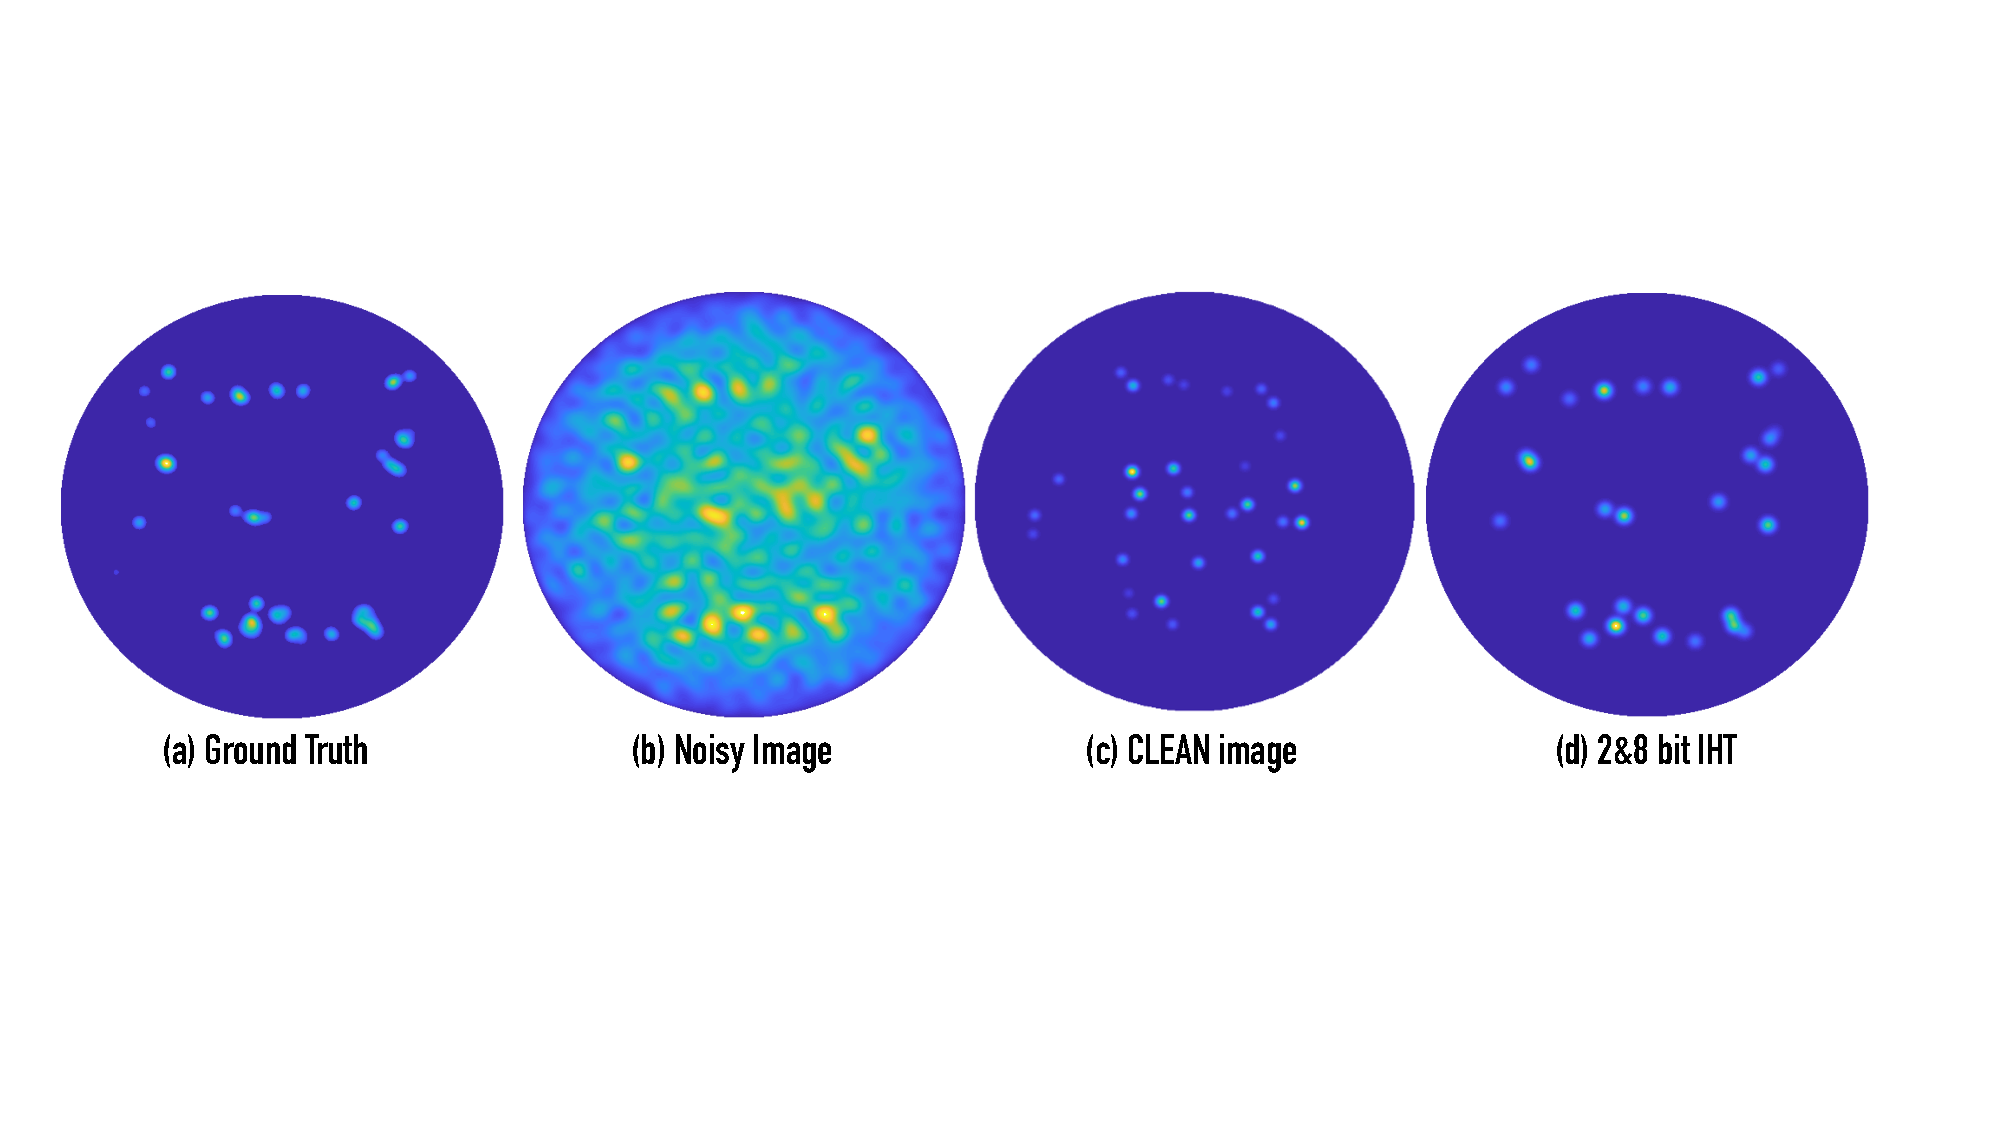
\includegraphics[width=1\columnwidth, angle=0]{figs/clean_image.pdf}
\caption{Comparison of 2\&8 bit IHT to CLEAN Algorithm. The CLEAN mostly captures the noise artefacts as actual sources unlike IHT.}
\label{fig:clean}
\end{figure}
Recall from the discussions in the main paper that noise in receivers is far stronger than the weak incoming signals thus low SNR at the antenna level results, i.e., usually ranged from -5 to 5 dB. In Fig., we apply the CLEAN algorithm to the LOFAR data set we use throughout the main paper, where SNR is computed nearly 0 dB. This particular experiment states that the CLEAN algorithm notably underperforms in the presence of significant noise. This undesirable property is yet not surprising. A careful look into the the algorithmic steps, it apparently matches also to the noise artefacts in the image considering them as a point source. This can also be justified mathematically: we designed the problem such that an execution of {CLEAN} corresponds to the first iteration recovery of IHT, which interprets our numerical results. 

Computationaly, the CLEAN requires a 2D Fourier inversion and deconvolution per iteration thus the operational expense of the method is relatively higher compared to those of IHT and CoSaMP. 

% \bibliography{references}
% \bibliographystyle{references}

\end{document}


% This document was modified from the file originally made available by
% Pat Langley and Andrea Danyluk for ICML-2K. This version was created
% by Iain Murray in 2018. It was modified from a version from Dan Roy in
% 2017, which was based on a version from Lise Getoor and Tobias
% Scheffer, which was slightly modified from the 2010 version by
% Thorsten Joachims & Johannes Fuernkranz, slightly modified from the
% 2009 version by Kiri Wagstaff and Sam Roweis's 2008 version, which is
% slightly modified from Prasad Tadepalli's 2007 version which is a
% lightly changed version of the previous year's version by Andrew
% Moore, which was in turn edited from those of Kristian Kersting and
% Codrina Lauth. Alex Smola contributed to the algorithmic style files.
